\section{Introduction}
\lorem

\section{Representation Extraction}
\lorem

\subsection{Manifold, Embedding and Neural Networks}
\lorem

\subsection{Dimensionality Reduction and Manifold Approximation}
\lorem

\section{Representation Analysis}
\lorem

\subsection{Joint Prediction Model}
\lorem

\subsection{Model Dynamic Prediction}
From figure \ref{pca_emb}A we can observe consistent patterns of cross-correlation for the activity of the artificial neurons constituting the RNN representation. This is supported by the fact that, considering only two dimensions, PCA was able to explain from 30 to 60\% of the variance in the representation generated by the RNN, with maximum explanatory power around 6 and 8 principal components.
\begin{figure}[h]
\centering
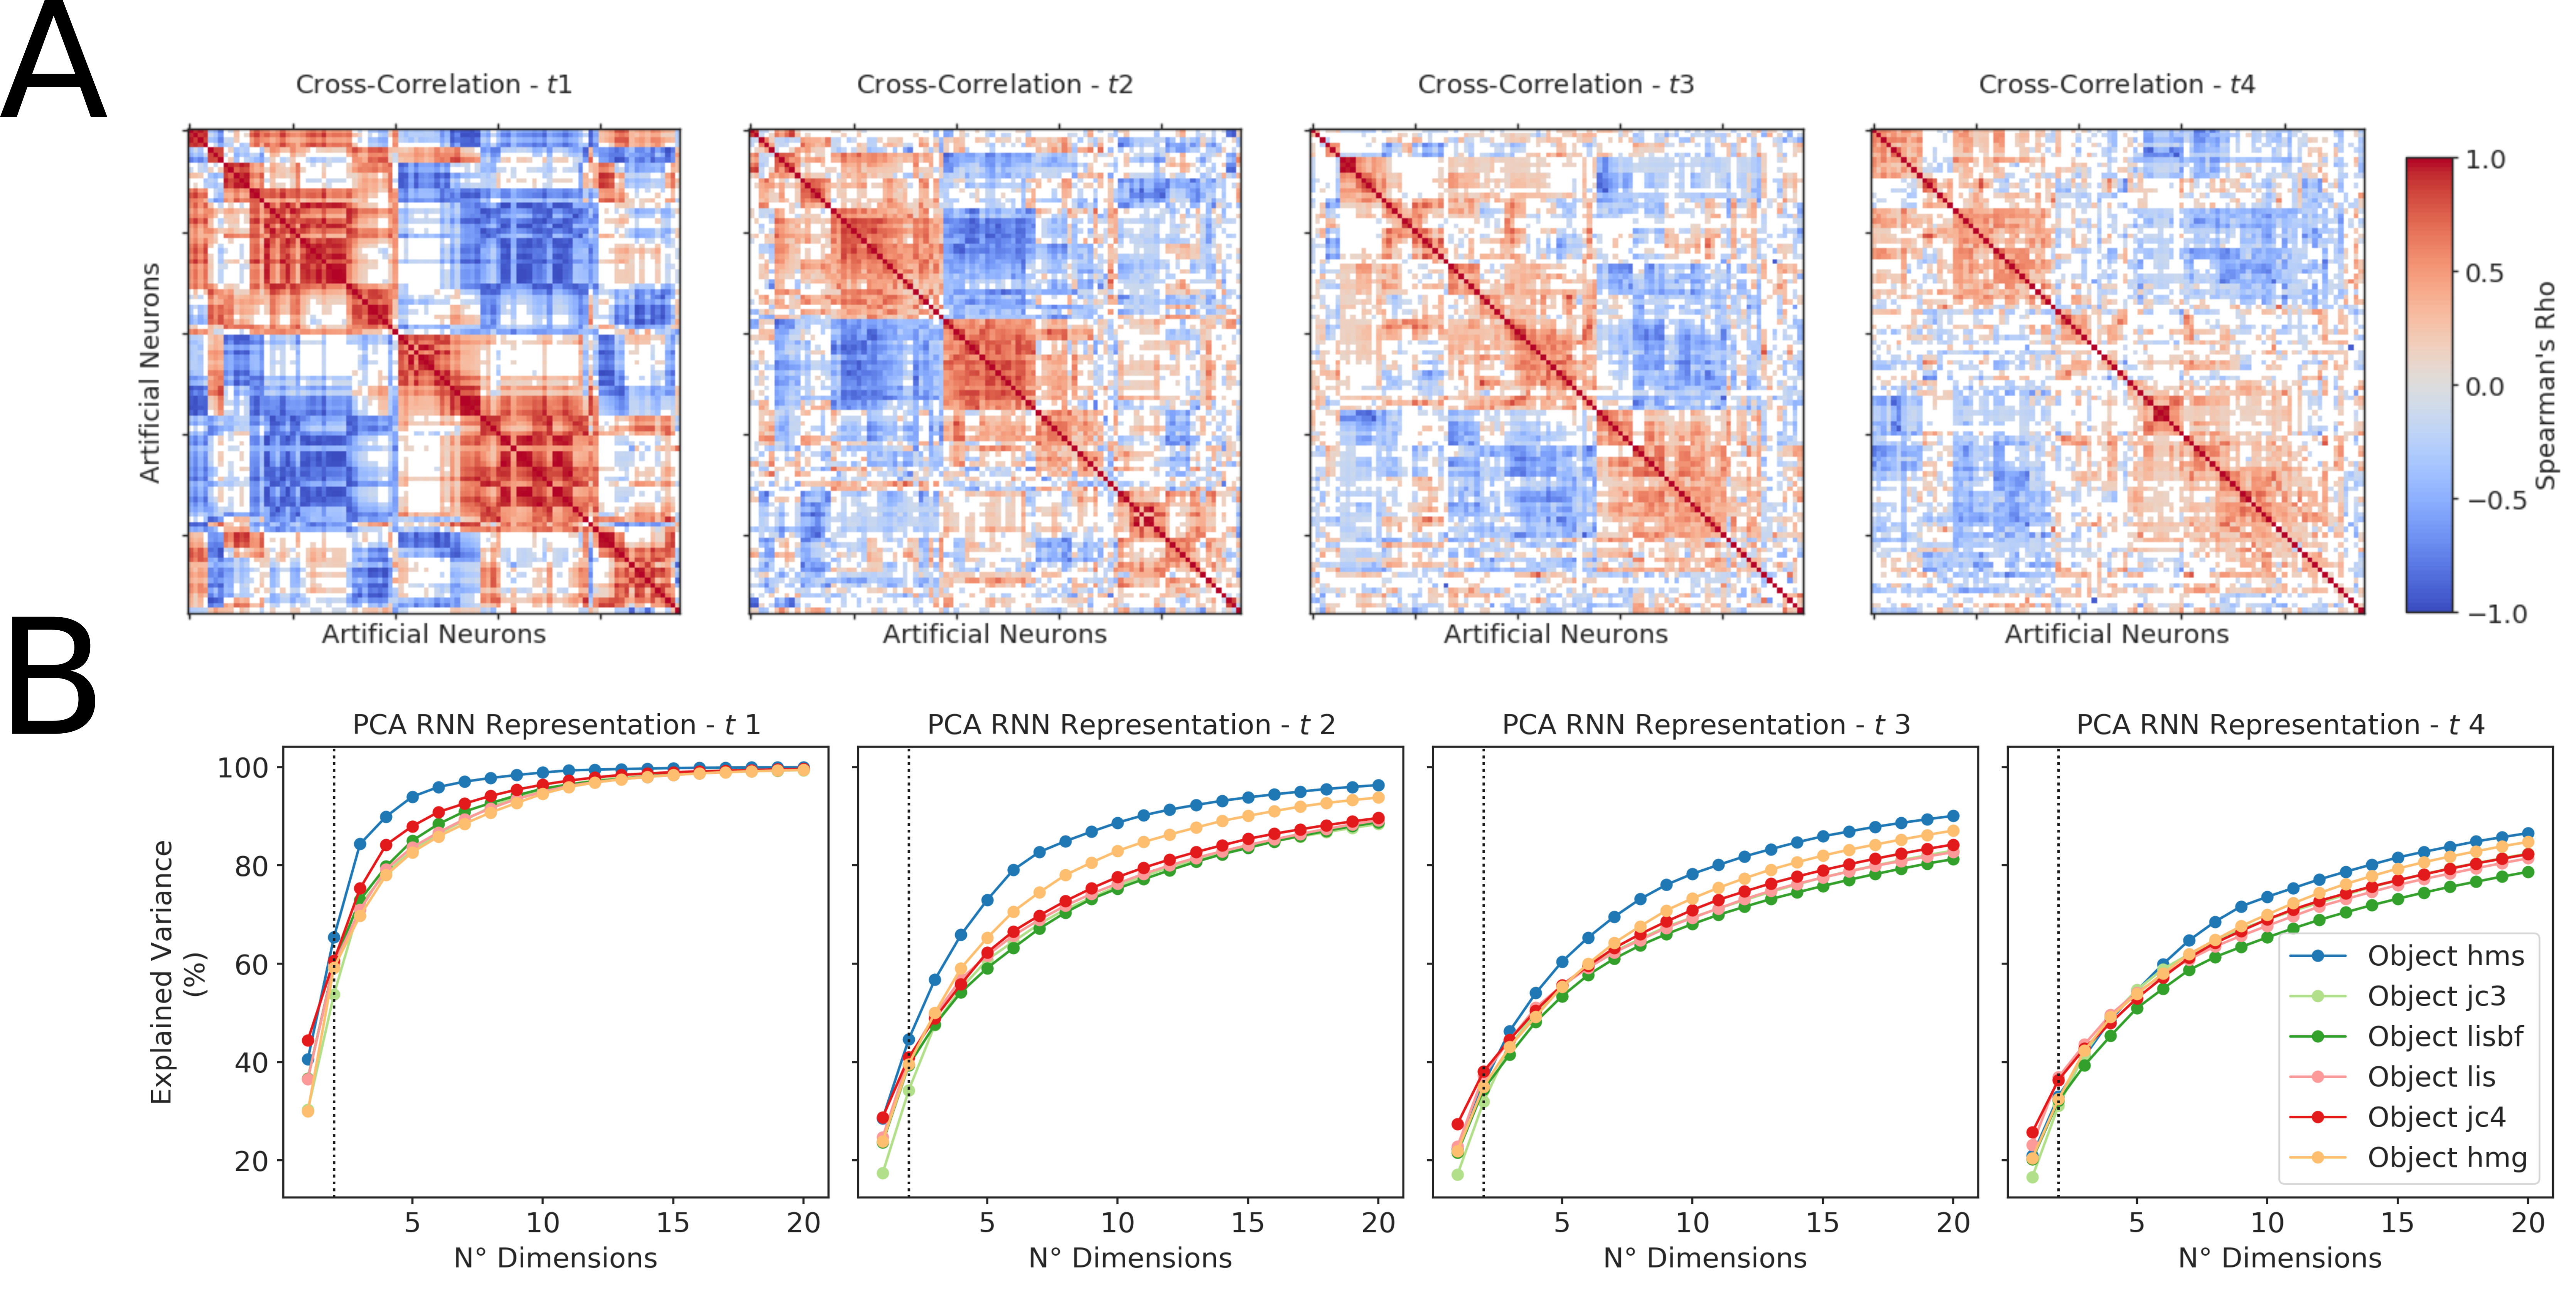
\includegraphics[width=0.8\textwidth]{images/chapter_4/pca_repr_42.png}
\caption[\textbf{Hidden units activation analysis of the RNN architecture}{The activity of the hidden units in the recurrent layer of the RNN architecture showed to be markedly redundant. Panel A shows the cross correlation between the activity of the RNN's artificial neurons in the game object $hms$ going from $t1$ to $t4$. The y and x axes are symmetrical and identifies the RNN artificial neurons while the coloured cells report the Spearman's Rho correlation coefficient for the activation of each pair of neurons. White cells represent combinations for which the correlation coefficient resulted lower than 0.05. \textbf{Two principal components can explain a large portion of variance in the representation generated by the RNN.} Panel B shows the percentage of explained variance by considering 2 to 20 principal components for each game object going from $t1$ to $t4$. The y axis indicates the percentage of explained variance while the x axis the number of principal components considered.}
\label{pca_emb} 
\end{figure}

Inspecting the representation generated by the RNN model at $t1$ (see Figure \ref{full_panel_static}A) we observe that the model was able to effectively distinguish between different game objects while simultaneously encoding for variations in the expected intensity of future interactions. This is illustrated by the fact that each game object occupies different and distinct regions in the representation space while showing a within-object gradient-like organization that places individuals (i.e. single dots) on a continuum based on the estimated magnitude of their future behaviour. This organization is preserved for each of the six targets showing how the representation inferred by the model is a suitable meta-descriptor for different behavioural indicators. As expected, some targets show a very similar but not identical organization (e.g. Future Session Time and Future Session Activity) while others appear to be independent (e.g. Future Session Time and Future Absence). We note that the absolute location of each game aggregate (i.e. all the points belonging to a specific game object) on the 2D plane is arbitrary. As we can see in figures \ref{full_panel_static} and \ref{full_panel_temporal}, this will change at every run of the algorithm due to the stochastic nature of UMAP. Panels \ref{full_panel_static}B and \ref{full_panel_static}C provide more insight into the activation profiles of individual hidden units constituting the generated representation. Panel \ref{full_panel_static}B shows the relationship between the activity of 10 randomly-chosen units and the predictions generated for the five targets. These are essentially transducer functions illustrating how the estimate for a particular target varies (on average) as the output of a units increases or decreases. Each unit seems to encode for multiple non-monotonic functions, one for each of the considered targets. Differences in the shape of these functions reflect similarities between their associated targets. For example, the functions associated to two highly related targets like Future Session Time and Future Session Activity (see panel \ref{full_panel_static}A) appear to be very similar in shape (see panels \ref{full_panel_static}B and \ref{full_panel_static}C). Interestingly, although most units appear to encode for unique functions some of them (e.g. 41 and 44) show an almost identical behaviour. This suggests the presence of redundancy in the functions underlying the representation generated by the RNN model. These observations are clarified in panel \ref{full_panel_static}C, where the functions associated with a single unit (20, indicated by a dark box in \ref{full_panel_static}B) are presented. Here we observe a strong, non-linear relationship between the unit's activity and the estimated targets (see the high MIC values and the line of best fit). In addition, the between-targets variation in MIC values suggest how the chosen unit is not equally informative for all targets.

\begin{figure}[ht]
\centering
\includegraphics[width=0.9\textwidth]{images/chapter_4/static_repr_42.png}
\caption{\textbf{The representation generated by the RNN model distinguishes between different game objects while maintaining an overarching organization able to capture variations in the expected intensity of future interactions that individuals will have with a specific game object}. Panel A shows the two-dimensional projection, produced by UMAP, of the multi-dimensional representation inferred by the RNN at $\mathbf{t1}$ as produced by UMAP. We can read the values of the x and y axes as a coordinate system where proximity represents similarity between points in the original high-dimensional space. Each point indicates the representation inferred by the RNN model after observing one game session from a single user. The colours in the Game Context panel indicate the game object from which the representation is coming. Colours in the small panels represent the discounted sum of all future predictions for a particular target (for example, estimated Future Session Time) $\widehat{B}_{t2:T}$ which is given by $\sum_{i=0}^{t2:T} \gamma^i\widehat{B_i}$ with $\gamma=0.1$ as illustrated in equation \ref{td_v}. \textbf{Each unit  encodes the intensity of future interactions through multiple non-monotonic functions}. Panels B and C show the relationship between the activation of randomly-selected hidden units in the LSTM layer of the RNN and the model's predictions at $\mathbf{t1}$. Panel B shows the relationship between the discretized activation of 10 randomly selected units (artificial neurons) plotted along the y axis and the predictions made by the model at $t1$ (colour coded from blue to red as in the small panels in A) for the game object $hmg$. Panel C shows in more detail the relationship between discretized activation and RNN predictions for a single unit highlighted by a black box in Panel B. Here the x axis indicates the discretized activation while the y axis the mean discretized discounted sum of all future predictions produced by the model. Vertical lines are standard errors of the mean. The red curve is the line of best fit provided by a generalized additive model \cite{serven2018} while the box reports the MIC and the correlation coefficient (Spearman's $\rho$) between the artificial neuron activation and the model's predictions.}
\label{full_panel_static}
\end{figure}
The analyses in Figure \ref{full_panel_static} were performed at a single time point $t1$. When performed at subsequent time points the results appear to be qualitatively similar. For example, focusing on Future Session Time (see Appendix \ref{appendix_representation} for results connected to other targets), we see in Figure \ref{full_panel_temporal}A that the model's ability to segregate different game objects while providing an  overarching representation of the intensity of future interactions is preserved over time. This supports the hypothesis that the representation inferred by our model is dynamic in nature which is further corroborated by panel \ref{full_panel_temporal}D. There we can see how the RNN model was able to individuate a "space" with temporally consistent ”hot” and ”cold” regions between which individuals moved over time depending on the expected intensity of their future interactions. This means that given the history of interaction of a particular individual with a specific game object, our model would determine their "position" (i.e. their "internal state") in the "attributed incentive salience space". This aligns with the manifold hypothesis mentioned in sections \ref{manifold_state} and \ref{manifold_learning}: changes in the propensity to interact with a specific game object (i.e. variations in the amount of attributed incentive salience) can be expressed moving on a manifold embedded within an $h$ dimensional space, with $h$ being the dimensionality of the representation generated by our RNN model. It appears that the hidden units constituting this representation tend to be consistent over time in the type of functions they encode (see Figure \ref{full_panel_temporal}B and C). As expected, we can again observe a strong non linear association between units' activation and targets' predictions, see MIC values and lines of best fit. The decrease in MIC value observed in Figure \ref{full_panel_temporal}C for the artificial neuron 72 might indicate how certain units lose their informative power over time.
\begin{figure}[ht]
\centering
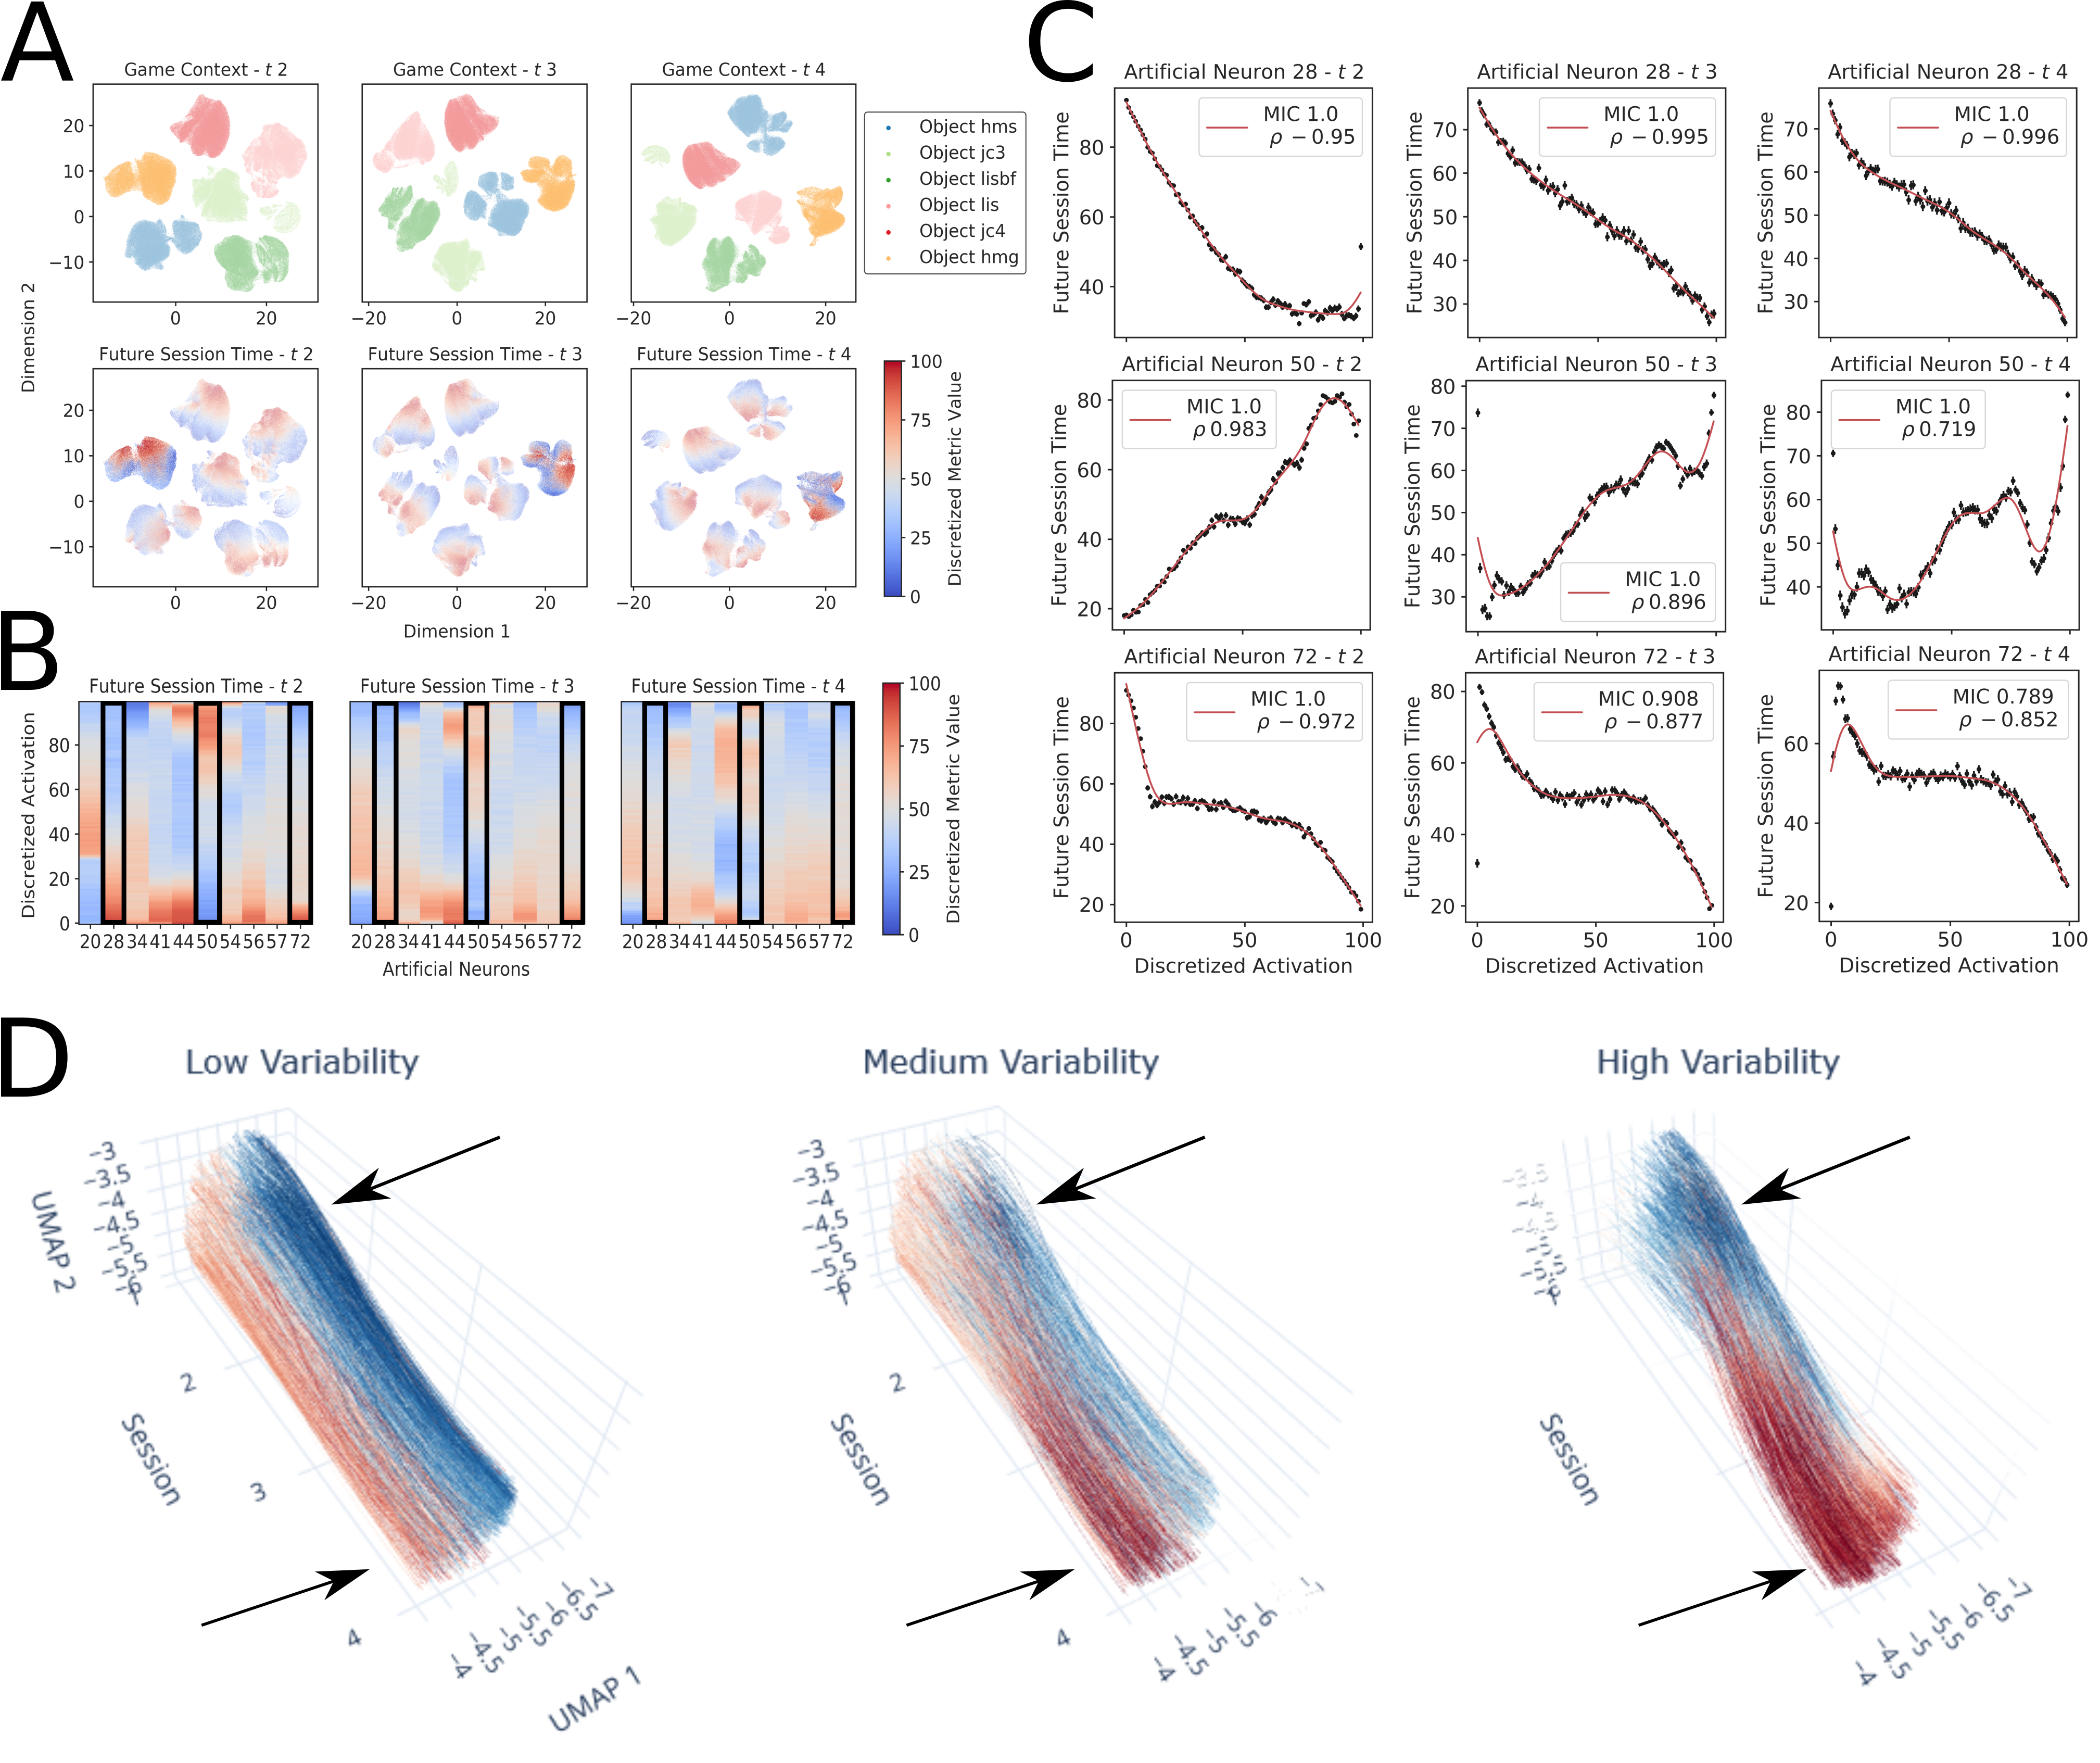
\includegraphics[width=0.9\textwidth]{images/chapter_4/dynamic_repr_42.png}
\caption{\textbf{The representation generated by the RNN model maintains its discriminant properties over time}. Panel A shows a two-dimensional projection of the multi-dimensional representation inferred by the RNN at $t2$, $t3$ and $t4$. The inferred representation maintains its gradient-like organization over time with an increased ability to differentiate between game objects. As in Figure \ref{full_panel_static}, x and y axes are dimensions individuated by the UMAP algorithm and can be interpreted as a coordinate system where proximity represents similarity between points. Colours in the first row indicate which game object the representation is coming from while those in the second row indicate the discounted sum of future predictions for a single target (i.e. "Future Session Time"). \textbf{The units constituting the generated representation encode for functions that are consistent over time.} Panels B and C show the relationship between units' activation and the model's predictions over time for the game object $hmg$. Different units appear to encode the same target with different non non-monotonic functions which are relatively consistent over time. Panel B illustrates the relationship between the same 10 randomly selected units specified in figure \ref{full_panel_static} and the predictions made by the model for Future Session Time at $t2$, $t3$ and $t4$. Panel C shows in more detail the relationship of the three artificial neurons, highlighted by black boxes in B, across time. Each row is a different unit while each column corresponds to a different $t$. The x axis indicates the discretized activation while the y axis the mean discretized discounted sum of all future predictions. Vertical lines are standard errors of the mean. The red curve is the line of best fit provided by a generalized additive model \cite{serven2018} while the box report the MIC and the correlation coefficient (Spearman's $\rho$) between the artificial neuron activation and the model's predictions. \textbf{The generated representation produces areas of low and high expected intensity among which individuals move over time.} Panel D shows trajectories through time produced by a version of UMAP that incorporates temporal information. Data are drawn from random subsets of individuals having low, medium and high variability in their expected amount of future behaviour. The representation inferred by the RNN model produces "hot" (i.e. the left side) and "cold" (i.e. the right side) regions, representing high and low expected Future Session Time, that are spatially consistent over time. Individuals appear to either stay in the same region or to move between regions over time. Here each line represents variations in the representation generated by the RNN model for a single user over four temporal steps. Continuity is generated by means of cubic spline interpolation for the lines and by linear interpolation for the colours. The x and y axes are the dimensions individuated by the UMAP algorithm while the z axis indicates the associated point in time. Colours indicate the discounted sum of future predictions produced by the model at a specific point in time.}
\label{full_panel_temporal}
\end{figure}

As we mentioned in section \ref{comp_framework}, both ANNs try to predict the intensity of future behaviour given the history of interactions. They do so relying on the same type of metrics, leveraging similar computational mechanisms (i.e. multitask learning and non-linearity) and producing representation according to the same underlying principle (i.e. the manifold hypothesis). Nevertheless, the fact that MLP provides poorer fit to data already suggests that whatever representation it has inferred it is likely a sub-optimal approximation of the manifold structure of incentive salience. Looking at figure \ref{predictive_panel}A, and knowing that UMAP represents differences and similarities between points through distance, we can see how the representation generated by the MLP less clearly differentiate between game objects. On the same figure, we can notice how the gradient representation for the metric Future N° Sessions Time is largely disrupted. This effect is however consistently less pronounced for other metrics (see our \href{https://htmlpreview.github.io/?https://github.com/vb690/approx_incentive_salience/blob/main/notebooks_html/embedding_analysis.html}{GitHub} for additional visualizations), in accordance to the differences we observed in predictive performance (see Figure \ref{model_comp_non_coll}). Recalling what mentioned in section \ref{comp_framework}, the latent state produced by the level of attributed incentive salience should retain at any point in time some predictive power over the intensity of all the future interactions (i.e. not just the one that follows). Figure \ref{rnn_future}B shows the representation generated by RNN and MLP at $t1$ but color coded with the discounted sum of the predictions made from $t4$ onward. We can see that, even if degraded, RNN still preserves some of the desired gradient-like organization which is instead much more disrupted for MLP. This is in accordance to what is shown by Figure \ref{full_panel_temporal}D: the RNN appears to define regions of high and low expected behavioural intensity which are consistent over time rather than constrained to the region around $t+1$.
\begin{figure}[ht]
\centering
\includegraphics[width=0.9\textwidth]{images/chapter_4/RNN_MLP_repr_42.png}
\caption{\textbf{The representation generated by the MLP model is less effective at distinguishing between different game objects and different levels of expected future behaviour intensity.}. Panel A shows a two-dimensional projection of the multi-dimensional representation inferred by the MLP at $t1$, $t2$, $t3$ and $t4$. Differently from the RNN, the representation shows a disruption in the gradient-like organization and a reduced ability to differentiate between game objects which remain constant over time. The x and y axes are dimensions individuated by the UMAP algorithm and can be interpreted as a coordinate system where proximity represents similarity between points. Colours in the first row indicate which game object the representation is coming from while those in the second row indicate the discounted sum of future predictions for a single target (i.e. "Future N° of Sessions") \textbf{The representation generated by the MLP model is less effective at at distinguishing different levels of expected behaviour intensity for states that are further away in the future.} Panel B shows a two-dimensional projection of the multi-dimensional representation inferred by the RNN (left) and MLP(right) at $t1$ but colour coded with the discounted sum of future predictions from $t4$ onward. The representation generated by the RNN is able to maintain a gradient-like organization even from states that are further away in the future while this capacity is almost entirely lost for the MLP. The colours in the Game Context panel indicate the game object from which the representation is coming. Colours in the small panels represent the discounted sum of all future predictions for a particular target computed from $t4$ onward instead that from $t1$. The x and y axes are the dimensions individuated by the UMAP algorithm.}
\label{predictive_panel}
\end{figure}

\subsection{Model Dynamic Prediction with Covariates}
\lorem

\section{Partition Analysis}
\lorem

\subsection{Joint Prediction Model}
\lorem

\subsection{Model Dynamic Prediction}
\lorem

\subsection{Model Dynamic Prediction with Covariates}
\lorem

\subsection{Discussion}
\lorem
